\documentclass[11pt]{article}
\usepackage[margin=0.78in]{geometry}
\usepackage{amsmath,amssymb,amsthm,mathtools}
\usepackage{graphicx}
\usepackage{xcolor}
\usepackage[hidelinks]{hyperref}
\usepackage{microtype}
\usepackage{booktabs}
\newtheorem{theorem}{Theorem}
\newcommand{\Ent}{\mathrm H}
\newcommand{\whT}{\widehat T_2}
\definecolor{accent}{RGB}{112,37,45}
\begin{document}
\begin{center}
{\Large\bfseries A Two-Phase Generalized Ewens Law Violates Every\\[2pt]
Source-Scale Transport--Entropy Bound}\par
\vspace{5pt}
{\small Counterexample to the parameter-uniform direct extension in
arXiv:1609.07315v3}\par
\end{center}

\noindent\colorbox{accent!10}{\parbox{0.96\linewidth}{\textbf{Status: candidate full counterexample.}
One explicit strictly positive generalized Ewens law on $S_{64}$ violates
each of the source inequalities (7), (8), and (9) with its stated constant.
The construction also explains why control uniform over arbitrary cycle
weights is impossible.}}

\section*{1. Exact question and the hidden hypothesis}
Samson~[1] asks whether its preceding transport--entropy inequalities extend
to generalized Ewens laws.  The tempting observation that these laws are
invariant under inversion and conjugation is insufficient: the opening of
Theorem 1.3 assumes $\mu\in\mathcal M_T$ for the entire theorem, and the proof
of part (b) uses the associated product disintegration.  The source itself
notes that generalized Ewens laws need not lie in $\mathcal M$.

\begin{center}
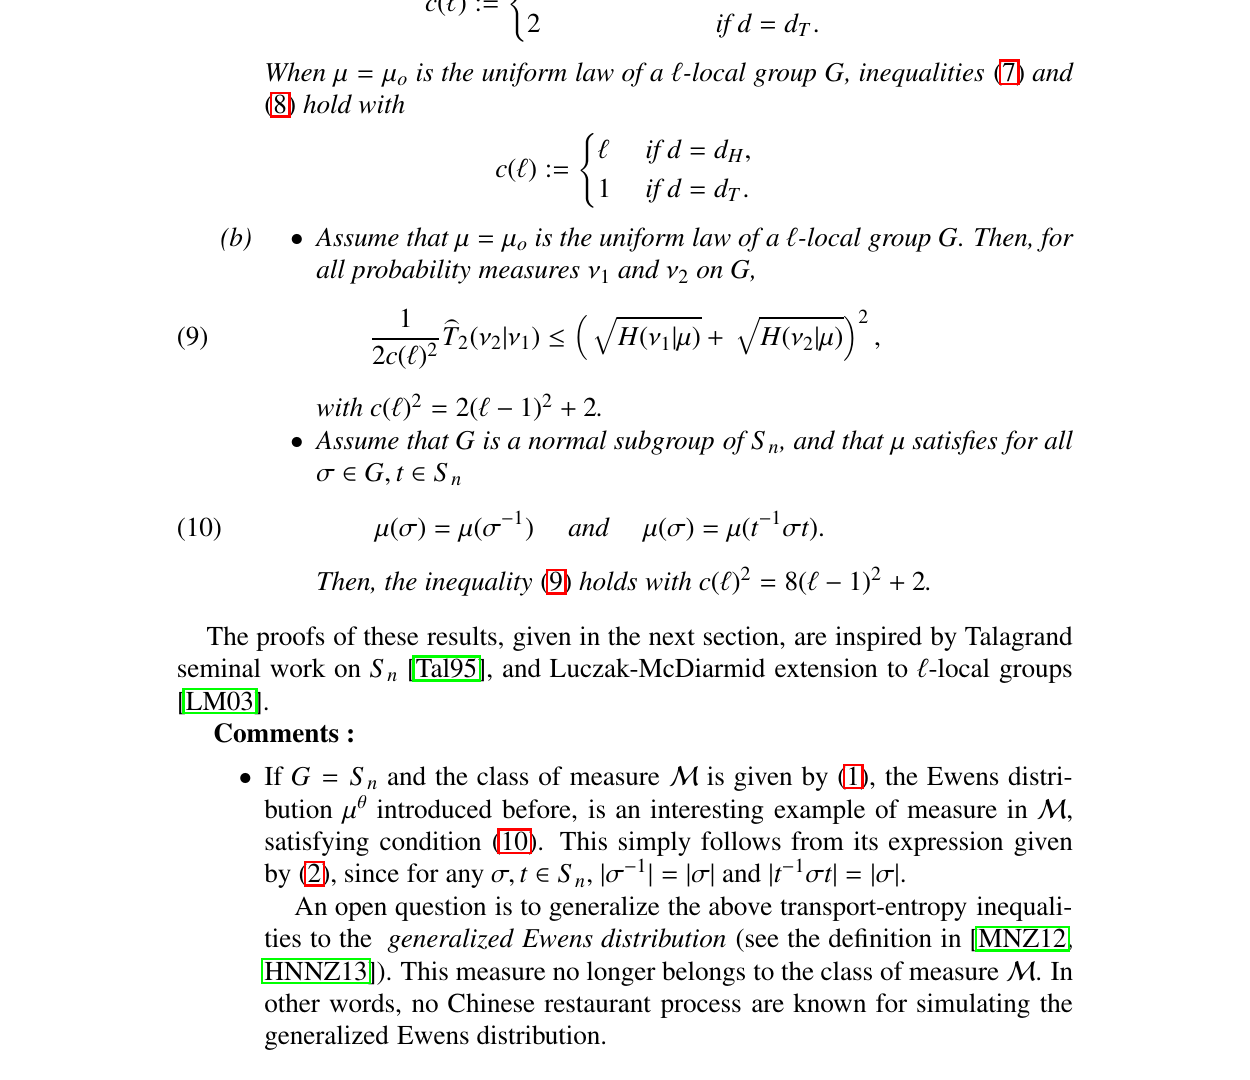
\includegraphics[width=.56\linewidth]{figures/theorem_and_question_crop.png}
\end{center}

\section*{2. Idea of the proof: an explicit two-phase law}
For generalized Ewens weights $\Theta=(\theta_k)_{k=1}^{64}$, put
\[
 \theta_1=1,\qquad
 \theta_k=10^{-200}\ (2\le k\le63),\qquad
 \theta_{64}=\frac1{63!},
\]
and let
\[
 \mu_\Theta(\sigma)=Z^{-1}\prod_{k=1}^{64}
 \theta_k^{C_k(\sigma)}\qquad(\sigma\in S_{64}).
\]
Every weight is strictly positive.  In unnormalized mass, the identity has
weight $1$.  There are $63!$ many $64$-cycles and each has weight $1/63!$,
so that conjugacy class also has total mass $1$.

Every remaining permutation contains at least one cycle of length in
$\{2,\dots,63\}$ and has raw weight at most $\varepsilon:=10^{-200}$.  If $r$
is the aggregate raw mass of all remaining permutations, then
\[
 0<r\le64!\,\varepsilon<10^{-100}<0.01,
 \qquad Z=2+r. \tag{1}
\]
Thus $\mu_\Theta$ is an almost exact half-mixture of the identity and the
uniform law on $64$-cycles.

\section*{3. Simultaneous failure of (7), (8), and (9)}
Take $\nu_1=\delta_e$ and $\nu_2=\mu_\Theta$.  The entropy expression on the
right of all two-measure inequalities is
\[
 E=\left(\sqrt{\Ent(\nu_1\mid\mu_\Theta)}+
 \sqrt{\Ent(\nu_2\mid\mu_\Theta)}\right)^2
 =\log(2+r)<\log(2.01)<0.7. \tag{2}
\]
Since the first marginal is a point mass, its coupling with $\mu_\Theta$ is
unique.  Every $64$-cycle moves all $64$ points and has transposition distance
$63$ from $e$.  Consequently
\begin{align}
 W_{1,H}&\ge\frac{64}{2+r}, &
 \widetilde T_{2,H}&=W_{1,H}^2,\tag{3}\\
 W_{1,T}&\ge\frac{63}{2+r}, &
 \widetilde T_{2,T}&=W_{1,T}^2,\tag{4}\\
 \whT(\nu_2\mid\nu_1)&\ge
 64\left(\frac1{2+r}\right)^2. &&\tag{5}
\end{align}
The last line follows because a $64$-cycle moves each fixed coordinate, with
probability at least $1/(2+r)$ under $\mu_\Theta$.

For $S_{64}$ one has $\ell=2$ and $K_n=63$.  In part (a), $c=3$ for Hamming
distance and $c=2$ for transposition distance.  The right side of (7) and (8)
is below $63(0.7)=44.1$.  Using only $r<0.01$, their left sides satisfy
\[
\begin{array}{c@{\qquad}c@{\qquad}c}
\text{source bound}&\text{cost}&\text{left side lower bound}\\ \toprule
(7)&W_{1,H}&\frac{2}{9}(64/2.01)^2>225\\
(7)&W_{1,T}&\frac{1}{2}(63/2.01)^2>491\\
(8)&\widetilde T_{2,H}&\frac{1}{18}(64/2.01)^2>56\\
(8)&\widetilde T_{2,T}&\frac{1}{8}(63/2.01)^2>122.
\end{array}
\]
Hence all four versions fail.

For the invariant-law constant in (9), $c(2)^2=8(2-1)^2+2=10$.  Equations
(2) and (5) give
\[
 \frac1{2c(2)^2}\whT(\nu_2\mid\nu_1)
 >\frac{64}{20(2.01)^2}>0.79>0.7>E,
\]
so (9) fails as well.  This proves the promised simultaneous counterexample.

\section*{4. Scope and stronger obstruction}
The counterexample refutes the direct extension with constants uniform over
all positive cycle weights.  Replacing $64$ by growing $n$ makes the squared
metric cost order $n^2$ while the entropy stays near $\log2$; hence the same
family defeats every parameter-independent $O(n)$ constant.

It does not preclude transport inequalities with constants depending on
$\Theta$, nor results under quantitative regularity assumptions on
$(\theta_k)$.  Such dependence is unavoidable: on a finite group every
positive law admits some finite constant, while arbitrary cycle weights can
create the separated phases above.

\section*{References}
{\raggedright
\noindent[1] P.-M. Samson, \emph{Transport-entropy inequalities on locally
acting groups of permutations}, arXiv:1609.07315v3, pp.~5--6.
\par}
\end{document}
